%% LyX 2.3.1 created this file.  For more info, see http://www.lyx.org/.
%% Do not edit unless you really know what you are doing.
\documentclass[12pt,english,letterpaper]{kuthesis}
%\usepackage{mathptmx}
\usepackage{amsmath}
\usepackage{amssymb}
\usepackage{amsthm}
\usepackage{commath}
\usepackage{lmodern}
%\usepackage{libertine,libertinust1math}
%\usepackage{concrete,eulervm}
%\usepackage{newpxtext,newpxmath}
%\usepackage{newtxtext,newtxmath}
%\renewcommand{\sfdefault}{lmss}
%\renewcommand{\ttdefault}{lmtt}
\usepackage[T1]{fontenc}
\usepackage[utf8]{inputenc}
\usepackage{geometry}
\geometry{verbose,tmargin=1in,bmargin=1in,lmargin=1in,rmargin=1in}
\setcounter{secnumdepth}{3}
\setcounter{tocdepth}{3}
\usepackage[dvipsnames]{xcolor}
\usepackage{babel}
\usepackage{url}
\usepackage{graphicx}
\usepackage{setspace}
\usepackage{esint}
\usepackage{siunitx}
\usepackage[authoryear]{natbib}
\doublespacing
\usepackage[unicode=true,
bookmarks=true,bookmarksnumbered=false,bookmarksopen=false,
breaklinks=true,pdfborder={0 0 0},pdfborderstyle={},backref=false,colorlinks=true]
{hyperref}
\hypersetup{pdftitle={Topological Optimization Using the SIMP Method},
	pdfauthor={Mikal Nelson},
	pdfsubject={Mathematical Optimization},
	urlcolor={black},citecolor={black},allcolors={black}}
\usepackage{jlcode}
\usepackage{algorithm}
\usepackage{algorithmicx}
\usepackage{algpseudocode}
\usepackage{tikz}
\usepackage{tikzit}
\input{thesis.tikzstyles}

\newcommand{\sref}[2]{\hyperref[#2]{#1 \ref{#2}}}

\makeatletter

%%%%%%%%%%%%%%%%%%%%%%%%%%%%%% LyX specific LaTeX commands.
\providecommand{\LyX}{\texorpdfstring%
	{L\kern-.1667em\lower.25em\hbox{Y}\kern-.125emX\@}
	{LyX}}
%% Because html converters don't know tabularnewline
\providecommand{\tabularnewline}{\\}

%%%%%%%%%%%%%%%%%%%%%%%%%%%%%% User specified LaTeX commands.

\newtheorem{thm}{Theorem}
\newtheorem{defn}{Definition}

%used to align decimals in tables according to APA style
\usepackage{dcolumn}
\usepackage{booktabs}

% Set the title and author info
\title{Topological Optimization Using the SIMP Method}
\author{Mikal William Nelson}

% Following is OPTIONAL list of previous degrees earned. 
% If there are more than 5 or so, then title pagelayout may become too crowded,
% depending on the number of committee members. 
\priorcreds{B.S. Mathematics, University of Minnesota, 2013}
% It is acceptable to delete \priorcreds if it is not desired on title page

\dept{Department of Mathematics}
\degreetitle{Master of Arts}
\papertype{Thesis} %or Thesis (Choose whatever word you want to put on p.2)

%% Committee member names are required for the title page. We make space
%% for as many as 7 members, with various roles/titles.
%% It is required to have 7 entries, even if some are empty for committee and role
\committee{Paul Cazeaux}{Mat Johnson}{Dionyssios Mantzavinos}{Yannan Shen}{}{}{}
\role{Chairperson}{}{}{}{}{}{}
%At Most 7 members allowed, last here is blank on purpose to demonstrate
%flexibility

%%BOTH dates must be included. 
\@printd@testrue
\datedefended{July 26, 2021}
\dateapproved{July, 2021}

%% These settings are now in the kuthesis.cls file, but users are free
% to customize. listings has great documentation online
%% When listings are used, break lines
%\lstset{
%    breaklines=true,  % sets automatic line breaking
%    breakindent=2em,
%    breakatwhitespace=true,  % sets if automatic breaks should
%   breakautoindent=true
%}

\@ifundefined{showcaptionsetup}{}{%
	\PassOptionsToPackage{caption=false}{subfig}}
\usepackage{subfig}
\makeatother

\usepackage{listings}
\renewcommand{\lstlistingname}{\inputencoding{latin9}Listing}

\begin{document}
	\begin{romanpages}
		
		\maketitle
		
		\begin{abstractlong}
			\addcontentsline{toc}{chapter}{Abstract}
			Insert Abstract Here
			
		\end{abstractlong}
		
		\begin{acknowledgements}
			%%if you want a "quote" environment for acknowledgements,
			%% use acknowledgements instead of acknowledgementslong
			\addcontentsline{toc}{chapter}{Acknowledgements}
			
			Dedicated to my mother, my first math teacher.
			
			Thank you to my wife, father, brothers, and all the teachers and professors who have helped me grow along the way.
			
		\end{acknowledgements}
		
		\tableofcontents{}
		
		\listoffigures
		
		%\listoftables
		
	\end{romanpages}
	
	\chapter*{Introduction}
	\addcontentsline{toc}{chapter}{Introduction}
	%\input{Introduction/Introduction}
	\chapter{Background}
	\section{PDE Discretization}
Multidimensional topological optimization problems often involve the use of partial differential equations (PDEs) which model the physical properties of the materials involved. Most of these PDEs cannot be uniquely solved analytically, so we turn to numerical methods in order to approximate their solutions. The first step in many of these methods is to discretize our domain; that is, we want to choose some scheme to divide our continuous domain into a finite number of pieces over which we will apply a particular method to approximate solutions to the PDE.

The implementation of the SIMP method introduced in $\S$\ref{sec:SIMP} uses the Finite Volume Method to discretize and approximate solutions to the heat equation for the heat generating medium. We will introduce the Heat Equation and then proceed to give an overview of the Finite Volume Method.
\subsection{The Heat Equation}
Consider heat flow through a stationary, inhomogeneous object. The temperature at any point in the interior of the object will depend on the spatial position chosen as well as the time we measure the temperature at that point. Therefore, the temperature ($T$) at any point in such an object is a function of both space ($\mathbf{x}$) and time ($t$) coordinates: $T(\mathbf{x},t)$.
Physical principles require that such a temperature function must satisfy the equation
\begin{equation}
	\frac{\partial T}{\partial t}=\nabla\cdot\left(k(\mathbf{x})\nabla T\right)\label{eqn:HeatEq},
\end{equation}
where $\nabla$ is the gradient operator and the function $k$ represents the thermal diffusivity at a point in our object.

Equation \eqref{eqn:HeatEq} is commonly referred to as the Heat or Diffusion Equation. If we were to have a constant thermal diffusivity throughout our object on a simple domain (such as a square or circle), it would be possible to analytically find a solution to this partial differential equation. However, as in the VP heat conduction problem, when $k$ is not constant we must turn to numerical methods to find approximate solutions for the function $T$.

\begin{figure}
	\centering
	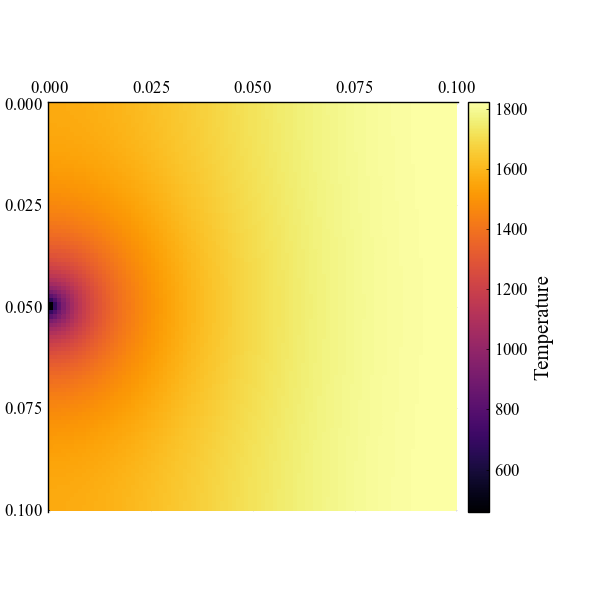
\includegraphics[width=0.8\textwidth]{Chapter_I_Background/Images/Heatmap_Example.png}
	\caption[Heatmap Example]{Heatmap for a \SI{0.1}{\meter} $\times$ \SI{0.1}{\meter} object with uniform heat generation and a heat-sink at the center of its west boundary. This map was produced via the Finite Volume Method using $100\times 100$ uniform control volumes.}
	\label{fig:heatmap-example}
\end{figure}

\subsection{The Finite Volume Method}\label{sec:FVM}

For the numerical approximations of PDEs in this paper the Finite Volume Method (FVM) was implemented, which will be described in this section.

As with many other numerical method to solve PDEs, we must first discretize our domain by creating a mesh. One major advantage of the finite volume method is that it allows for a great amount of freedom in mesh choice. When using FVM the domain can be discretized into a mesh of arbitrary polygons, but uniform squares or rectangles were chosen in our work to simplify the resulting calculations.

Given a mesh of polygons on a domain $\Omega$ with sample points at $\lbrace x_i\rbrace\subset\Omega$, we create a set of \textit{control volumes} around each $x_i$. The resulting set of control volumes will be used to discretize the partial differential equation. The finite volume method has us integrate our PDE over each control volume and then use the Divergence Theorem (\sref{Theorem}{thm:div-thm}) to convert volume integrals into surface integrals involving the fluxes across the boundaries of the control volumes. We then approximate those fluxes across the boundaries to calculate approximate solutions to the PDE of interest, such as \eqref{eqn:HeatEq}.

\begin{thm}[The Divergence Theorem]
	Suppose that $\mathcal{V}$ is a compact subset of $\mathbb{R}^n$ that has a piecewise smooth boundary $\mathcal{S}$ (i.e. $\partial\mathcal{V}=\mathcal{S}$) with outward pointing normal vectors. If $\mathbf{F}$ is a continously differentiable vector field defined on a neighborhood of $\mathcal{V}$, then
	\begin{equation}
		\iiint_{\mathcal{V}}\left(\nabla\cdot\mathbf{F}\right)\dif\mathcal{V}=\oiint_{\mathcal{S}}\left(\mathbf{F}\cdot\mathbf{\hat{n}}\right)\dif\mathcal{S}\label{eqn:div-thm}
	\end{equation}
	where $\hat{\mathbf{n}}$ is the outwards pointing normal vector to the boundary.
	\label{thm:div-thm}
\end{thm}

The divergence theorem is the key component in the finite volume method because it allows us to look at fluxes across the boundaries of each control volume, rather than the control volume itself.

Let us look at the finite volume method applied to the heat equation in two dimensions. Suppose we have discretized our space by dividing it up into a mesh of control volumes $\lbrace V_i\rbrace$. We integrate \eqref{eqn:HeatEq} over each control volume, using the divergence theorem to convert the volume integral into a surface integral:

\begin{equation}
	\int_{V_i}\frac{\partial T}{\partial t}\dif\mathbf{x}=\int_{V_i}\nabla\cdot \left(k(\mathbf{x})\nabla T\right)\dif\mathbf{x}\underset{\eqref{eqn:div-thm}}{=}\int_{\partial V_i}k(\mathbf{x})\nabla T\cdot\hat{\mathbf{n}}\dif s,\label{eqn:Vol-to-Surface-FVM}
\end{equation}

\noindent where $s$ represents the curves that form the boundary of the control volume. Then, applying an approximation scheme to this result, we obtain a sparse and structured linear system. For example, one could apply what is called a ``two-point flux approximation'' scheme which uses finite differences of function values from neighboring cells to the control volume to approximate the flux through the control volume faces \cite{Versteeg2007}.

In a square grid there are only four neighboring cells which we can label as North, South, East, West. For a control volume $V_i$ we'll label the North boundary as $\partial V_N$, the South boundary as $\partial V_S$, the East boundary as $\partial V_E$, and the West boundary as $\partial V_W$. Additionally, let $\Delta x$ be the length of the North and South boundaries, and $\Delta y$ the length of the East and West boundaries. We can discretize \eqref{eqn:Vol-to-Surface-FVM} as
\begin{equation}
	\begin{tabular}{ccc}
		$\displaystyle\int_{\partial V_i}k(\mathbf{x})\nabla T\cdot\hat{\mathbf{n}}\dif s$ & $=$ & $\displaystyle\int_{\partial V_N}k(\mathbf{x})\nabla T\cdot\hat{\mathbf{n}}_N\dif s+\int_{\partial V_S}k(\mathbf{x})\nabla T\cdot\hat{\mathbf{n}}_S\dif s$\\
		 &  & $\displaystyle+\int_{\partial V_E}k(\mathbf{x})\nabla T\cdot\hat{\mathbf{n}}_E\dif s+\int_{\partial V_W}k(\mathbf{x})\nabla T\cdot\hat{\mathbf{n}}_W\dif s$\\
		 & & \\
		 & $\approx$ & $\displaystyle k_N\frac{T_N-T_i}{\|\mathbf{x}_N-\mathbf{x}_i\|}\Delta x+k_S\frac{T_S-T_i}{\|\mathbf{x}_S-\mathbf{x}_i\|}\Delta x$\\
		 & & $\displaystyle+k_E\frac{T_E-T_i}{\|\mathbf{x}_E-\mathbf{x}_i\|}\Delta y+k_W\frac{T_W-T_i}{\|\mathbf{x}_W-\mathbf{x}_i\|}\Delta y$\\
		 & & \\
		 $\displaystyle\implies \Delta x\Delta y\frac{\dif T_i}{\dif t}$ & $=$ & $\displaystyle\left( k_N\frac{T_N-T_i}{\|\mathbf{x}_N-\mathbf{x}_i\|}+k_S\frac{T_S-T_i}{\|\mathbf{x}_S-\mathbf{x}_i\|}\right)\Delta x$\\
		 & & $\displaystyle+\left(k_E\frac{T_E-T_i}{\|\mathbf{x}_E-\mathbf{x}_i\|}+k_W\frac{T_W-T_i}{\|\mathbf{x}_W-\mathbf{x}_i\|}\right)\Delta y$
	\end{tabular}\label{deriv:descrete-FVM}
\end{equation}

The process in \eqref{deriv:descrete-FVM} is repeated for all control volumes $i$ to produce a system of ordinary differential equations which is used to solve for the values of $T_i$.

One other major advantage of the finite volume method is that boundary conditions can easily be taken into account on general domains. For example, adding a heat-sink by applying a Dirichlet boundary condition can be thought of as zeroing out our algebraic equations by introducing a ghost cell that, when interpolated with the boundary cell, causes the temperature across the boundary to be zero.
	\section{The Optimization Problem}

In much of mathematics, our goal is to seek some sort of solution. In cases where there are multiple solutions, it is desirable to determine the ``best'' solution judged against some set of criteria. Mathematical optimization is the study of solving such problems. In its simplest case, mathematical optimization is the practice of minimizing or maximizing a given function over a certain set and possibly subject to some constraints.

\begin{defn}
An {\color{tiananmen}optimization problem} (in standard form) has the form
\begin{equation}
	\begin{tabular}{lll}
		\text{minimize }   & $f_0(x)$          & \\
		\text{subject to } & $f_i(x)\leq 0$, & $i=1,\ldots, m$\\
		& $h_i(x) = 0$,      & $i=1,\ldots, p$
	\end{tabular}\label{Optimization}
\end{equation}
where
\begin{itemize}
	\item {\color{baystate} $x=\left(x_1,\ldots,x_n\right)$} are the {\color{tiananmen} \textbf{optimization variables}},
	\item {\color{baystate} $f_0 : \mathbb{R}^n\rightarrow\mathbb{R}$} is the {\color{tiananmen} \textbf{objective function}},
	\item {\color{baystate} $f_i : \mathbb{R}^n\rightarrow\mathbb{R}$} are the {\color{tiananmen} \textbf{inequality constraint functions}}, and
	\item {\color{baystate} $h_i : \mathbb{R}^n\rightarrow\mathbb{R}$} are the {\color{tiananmen}\textbf{equality constraint functions}}.
\end{itemize}
\end{defn}
If there are no constraints ($m=p=0$), then the problem is called {\color{tiananmen}\textit{unconstrained}}. \cite[p. 127]{Boyd2004}

We call a vector {\color{baystate} $x^\star$} {\color{tiananmen} \textbf{optimal}} if it has the smallest objective value among all vectors that satisfy the constraints. That is, for any $z$ with $f_1(z)\leq 0,\ldots, f_m(z)\leq 0$, then $f_0(z)\geq f_0(x^\star)$. A point $x$ that is in the domains of each function $f_i$ and $h_i$ is called {\color{tiananmen}\textbf{feasible}} if it satisfies all the constraints. Finally, the {\color{tiananmen} \textbf{optimal value}} {\color{baystate}$p^\star$} of the problem is defined as {\color{baystate}$$p^\star=\left\lbrace f_0(x) \mid f_i(x)\leq 0, i=1,\ldots,m, h_i(x)=0, i=1,\ldots,p\right\rbrace.$$} Therefore, $p^{\star}=f_0(x^\star)$, the objective function value at a feasible, optimal vector $x^{\star}$.

Notice that the optimization problem in standard form is a minimization problem.  We can easily change it into a maximization problem by minimizing the objective function $-f_0$ subject to the same constraints.

The optimization problem is {\color{tiananmen}\textbf{linear}} or called a {\color{tiananmen}\textbf{linear program}} if the objective and constraint functions are all linear. An optimization problem involving a quadratic objective function and linear constraints is {\color{tiananmen}\textbf{quadratic}} or a {\color{tiananmen}\textbf{quadratic program}}. If the optimization problem is not linear or quadratic, it is referred to as a {\color{tiananmen}\textbf{nonlinear program}}.

There are exists efficient methods for solving linear programming and many quadratic programming problems.

\subsection{Convex Optimization}

A set {\color{baystate}$C$} is {\color{tiananmen}\textbf{convex}} if the line segment between any two points in $C$ lies in $C$. That is {\color{baystate}if for any $x_1,x_2\in C$ and any $\theta$ with $0\leq\theta\leq 1$, we have $\theta x_1+(1-\theta)x_2\in C$}.

A function {\color{baystate}$f : \mathbb{R}^n\rightarrow\mathbb{R}$} is {\color{tiananmen}\textbf{convex}} if the domain of $f$ is a convex set and if for all $x,y$ in the domain of $f$, and $\theta$ with $0\leq\theta\leq 1$, we have
{\color{baystate}
	\begin{equation}
		f\left(\theta x+\left(1-\theta\right)y\right)\leq\theta f(x)+(1-\theta)f(y).
		\label{Convexity}
	\end{equation}
}
A {\color{tiananmen} \textbf{convex optimization problem}}, therefore, is an optimization problem of the form
{\color{baystate}
	\begin{equation}
		\begin{tabular}{lll}
			\text{minimize }   & $f_0(x)$          & \\
			\text{subject to } & $f_i(x)\leq 0$, & $i=1,\ldots, m$\\
			& $a_i^T = b_i$,      & $i=1,\ldots, p$
		\end{tabular}\label{ConvexOptimization}
	\end{equation}
	where $f_0,\ldots,f_m$ are convex functions.
}

There are three additional requirements that differentiate a convex optimization problem from a general optimization problem:
{\color{baystate}
	\begin{itemize}
		\item the objective function must be convex
		\item the inequality constraint functions must be convex
		\item the equality constraint functions must be {\color{tiananmen}\textbf{affine}}
	\end{itemize}
}

In a convex optimization problem we minimize a convex objective function over a convex set.

\textbf{In a convex optimization problem, any {\color{tiananmen}\textbf{locally optimal point}} is also {\color{tiananmen}\textbf{globally optimal}}.}
	\section{Optimization Methods}

In this section I will present a few optimization algorithms for unconstrained optimization.

These algorithms follow a general blueprint:
\begin{enumerate}
	\item Choose an initial ``guess'' for the optimal value $x$
	\item Find a Descent Direction $\Delta x$
	\item Use a line search method to determine an appropriate step-size ($t$) in the descent direction
	\item Compute new guess value: $x+t\Delta x$
\end{enumerate}

Each method uses a line search, but gow the descent direction is chosen is the main differentiating factor in each method.

\subsection{Line Search Methods}

The \textit{line search} is a strategy that selects the step size (commonly represented by $t$) that determines where along the line $\left\lbrace x+t\Delta x\mid t\in\mathbb{R}_+\right\rbrace$ the next iterate in the descent method will be. ($\Delta x$ represents the \textit{descent direction}, .) Line search strategies can either be \textit{exact} or \textit{inexact}.

\subsubsection*{Exact Line Search}

An \textit{exact line search} chooses the value $t$ along the ray $\left\lbrace x+t\Delta x\mid t\in\mathbb{R}_+\right\rbrace$ that exactly minimizes the function of interest $f$:
$$t=\arg\min_{s\geq 0}f(x+s\Delta x)$$
An exact line search is almost never practical. In very special cases, such as some quadratic optimization problems where an explicit formula is available, one might employ an exact line search.

\subsubsection*{Backtracking Line Search}
Most often in practice we use \textit{inexact line searches}. In an inexact line search, we choose $t$ such that $f$ is \textit{approximately} minimized or reduced ``enough'' along $\left\lbrace x+t\Delta x\mid t\in\mathbb{R}_+\right\rbrace$.

One inexact line search strategy is the \textit{Backtracking Line Search}.
\begin{algorithm}[H]
	\caption{Backtracking Line Search \cite{Boyd2004}\label{BacktrackingLineSearchAlg}}
	\begin{algorithmic} 
		\State \textbf{given} a descent direction $\Delta x$ for $f$ at $x\in\textbf{dom}f,\alpha\in(0,0.5),\beta\in(0,1)$.
		\State $t:=1$.
		\While{$f(x+t\Delta x)>f(x)+\alpha t\nabla f(x)^T\Delta x$}
		\State $t:=\beta t$
		\EndWhile
	\end{algorithmic}
\end{algorithm}

``Backtracking'' in the name is refers to the fact that the method starts with a unit step size $(t=1)$ and then reduces the step size (``backtracks'') by the factor $\beta$ until we meet the stopping criterion $f(x+t\Delta x)\leq f(x)+\alpha t\nabla f(x)^T\Delta x$.

%%% Need to reproduce image on own or something for final draft...

%Figure 9.1 \cite[p. 465]{Boyd2004} demonstrates the Backtracking Line Search visually for a parabola.
%\begin{center}
%	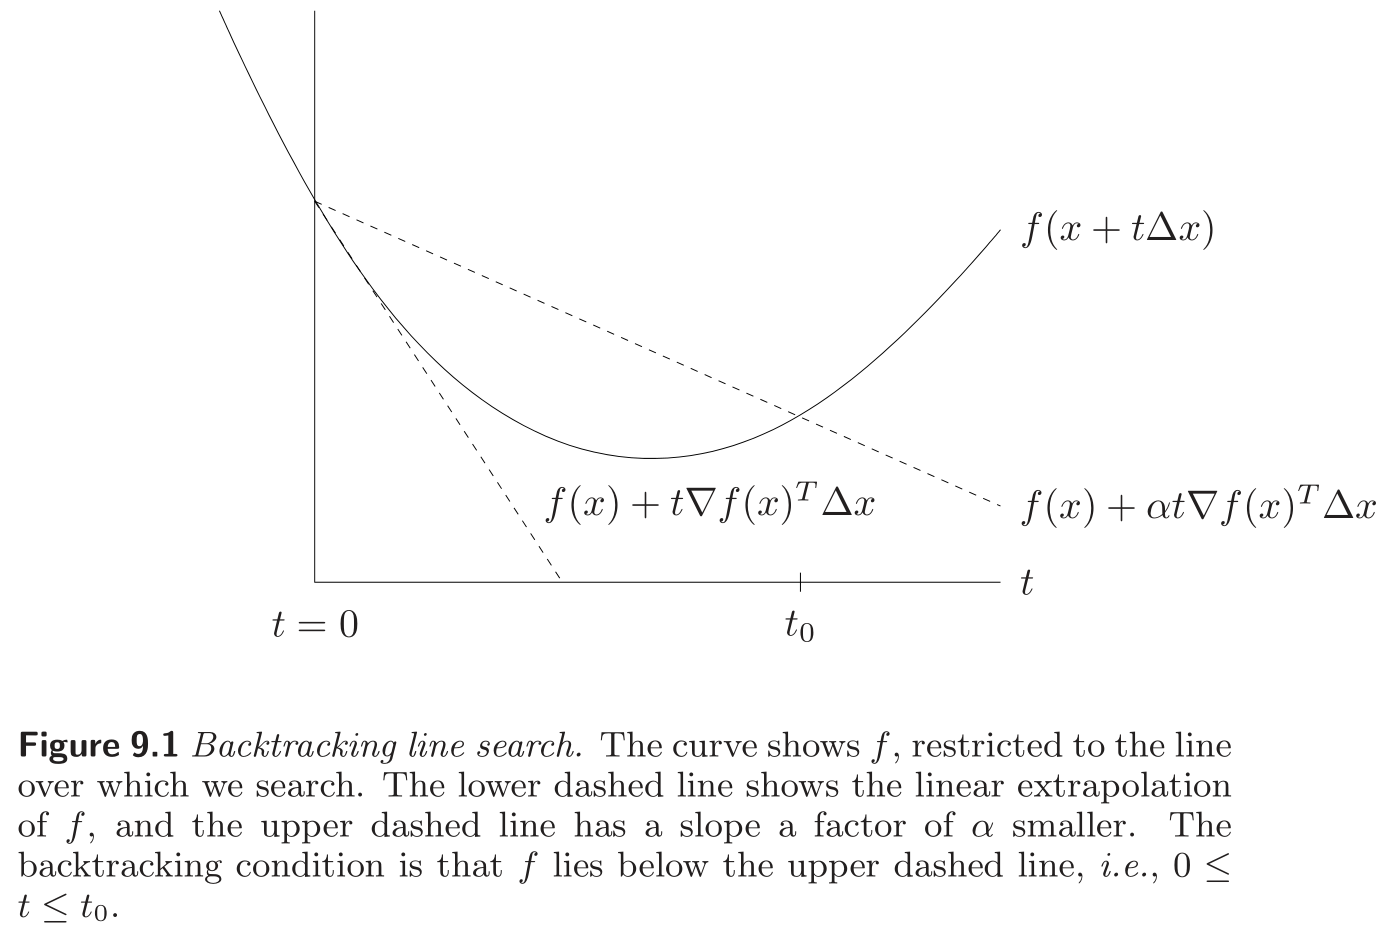
\includegraphics[width=0.75\textwidth]{Chapter_I_Background/Images/backtracking_line_search_diagram.png}
%\end{center}

Notice that the backtracking search will find a step size $t$ such that $0\leq t\leq t_0$ and that for such $t$, $f(x+t\Delta x)$ is smaller relative to $f(x)$. However, the step size we choose may not exactly be the minimum of the function, but we have funneled it down to be closer to the minimum of $f$.
\subsection{Gradient Descent}

The gradient descent method chooses the search direction to be the negative gradient. That is, in this method we set $\Delta x=-\nabla f(x)$, where $f$ is the function we seek to optimize. Since the gradient of a function gives the direction of greatest increase, naturally the negative gradient will give the direction of the most rapid decline.

\begin{algorithm}
	\caption{Gradient Descent Method \cite{Boyd2004}\label{GradientDescentAlg}}
	\begin{algorithmic} 
		\State \textbf{given} a starting point $x\in\textbf{dom}f$.
		\Repeat
		\begin{enumerate}
			\item $\Delta x:=-\nabla f(x)$.
			\item \textit{Line search.} Choose step size $t$ via exact or backtracking line search.
			\item \textit{Update.} $x:=x+t\Delta x$.
		\end{enumerate}
		\Until{stopping criterion is satisfied.}
	\end{algorithmic}
\end{algorithm}

Notice in Algorithm \ref{GradientDescentAlg} that essentially a line search is used to determine a step size and then we update our iterate in the direction of the steepest descent. This is repeated until we meet some sort of stopping criterion, typically something of the form $\|\nabla f(x)\|_2\leq\eta$, where $\eta$ is small and positive. Another common stopping criterion is to stop the algorithm when no significant progress is made between iterates by stopping the algorithm when $\|f_{k+1}-f_{k}\|<\eta$.

An implementation of the gradient descent algorithm in the Julia language can be found in the appendix.

\subsection{Nonlinear Conjugate Gradient}

The Nonlinear Conjugate Gradient method works similarly to the gradient descent algorithm, but adds the additional requirement that in each iteration gradient is orthogonal to each previous search direction.

Suppose we have a function $f(x)$ of $N$ variables. Let $x_0$ be an initial guess value for the minimum. The opposite of the gradient will give the direction of steepest descent. Therefore, we start off by setting $\Delta x_0=-\nabla f(x_0)$.

We set an adjustable step length $\alpha$ and perform a line search in the direction $d_0=\Delta x_0$ until a minimum of $f$ is reached:
\begin{align*}
	& \alpha_0:=\arg\min_{\alpha} f(x_0+\alpha\Delta x_0), \\
	& x_1=x_0+\alpha_0\Delta x_0.                          
\end{align*}

Suppose we were to simply iterate this process and for each step $i$ we do the following:

\begin{enumerate}
	\item Set $\Delta x_i=-\nabla f(x_i)$
	\item Calculate $\alpha_i=\arg\underset{\alpha}{\min}\ f(x_i+\alpha\Delta x_i)$
	\item Compute $x_{i+1}=x_i+\alpha_i\Delta x_i$
\end{enumerate}

However, there is an issue with this proposed iterative scheme: We have moved $\alpha_i$ in direction $\Delta x_i$ to find the minimum value in that direction, but by moving $\alpha_{i+1}$ in direction $\Delta x_{i+1}$ we may have accidentally \textit{undone} the progress made in the previous iteration so that we no longer have a minimum value in direction $\Delta x_i$. We can fix this problem by making sure that successive direction vectors have no influence in the directions of previous iterations. That is, we require our directions in each iteration to be conjugate (with respect to the matrix of coefficient for our system) to one another. Therefore, rather than taking $\Delta x_{i+1}$ to be $-\nabla f(x_i)$, we compute a direction conjugate to all previous directions by some pre-chosen methodology. This suggests the following iterative scheme:

After the first iteration, the following steps constitute one iteration along a conjugate direction:
\begin{enumerate}
	\item Calculate the new steepest descent direction: $\Delta x_i=-\nabla f(x_i)$,
	\item Compute $\beta_i$ using some formulation. Two options are below:
	\begin{itemize}
		\item Fletcher--Reeves: $\beta_i^{FR}=\frac{\Delta x_i^T\Delta x_i}{\Delta x_{i-1}^T\Delta x_{i-1}}$
		\item Polak--Ribi\`{e}re: $\beta_{i}^{PR}=\frac{\Delta x_i^T(\Delta x_i-\Delta x_{i-1})}{\Delta x_{i-1}^T\Delta x_{i-1}}$
	\end{itemize}
	\item Update the conjugate direction: $d_i=\Delta x_i+\beta_i d_{i-1}$,
	\item Line search: Optimize $\alpha_i =\arg\underset{\alpha}{\min}\ f(x_i+\alpha d_i)$,
	\item Update iterate value: $x_{i+1}=x_i+\alpha_i d_i$.
\end{enumerate}

Algorithm \ref{CongGradAlg} uses the Newton-Raphson method to find the values of $\alpha_i$.

\begin{algorithm}
	\caption{Nonlinear Conjugate Gradient Using Newton-Raphson \cite{Shewchuk1994}\label{CongGradAlg}}
	Given a function $f$, a starting value $x$, a maximum number of CG iterations $i_{\text{max}}$, a CG error tolerance $\epsilon<1$, a maximum number of Newton-Raphson iterations $j_{\text{max}}$, and a Newton-Raphson error tolerance $\varepsilon<1$:
	\begin{algorithmic}
		\State $i\Leftarrow 0$
		\State $k\Leftarrow 0$
		\State $r\Leftarrow -f^{\prime}(x)$
		\State $d\Leftarrow r$
		\State $\delta_{\text{new}}\Leftarrow r^Tr$
		\State $\delta_0\Leftarrow\delta_{\text{new}}$
		\While{$i<i_{\max}$ and $\delta_{\text{new}}>\epsilon^2\delta_0$}
		\State $j\Leftarrow 0$
		\State $\delta_d\Leftarrow d^Td$
		\While{true}
		\State $\alpha\Leftarrow -\frac{\left[f^{\prime}(x)\right]^Td}{d^Tf^{\prime\prime}(x)d}$
		\State $x\Leftarrow x+\alpha d$
		\State $j\Leftarrow j+1$
		\State $j<j_{\text{max}}$ and $\alpha^2\delta_d>\varepsilon^2$ OR \textbf{Break}
		\EndWhile
		\State $r\Leftarrow -f^{\prime}(x)$
		\State $\delta_{\text{old}}\Leftarrow\delta_{\text{new}}$
		\State $\delta_{\text{new}}\Leftarrow r^T r$
		\State $\beta\Leftarrow\frac{\delta_{\text{new}}}{\delta_{\text{old}}}$
		\State $d\Leftarrow r+\beta d$
		\State $k\Leftarrow k+1$
		\If{$k=n$ or $r^T d\leq 0$}
		\State $d\Leftarrow r$
		\State $k\Leftarrow 0$
		\EndIf
		\State $i\Leftarrow i+1$
		\EndWhile
	\end{algorithmic}
\end{algorithm}

%To get some intuition of how this algorithm operates, let's look at it applied to a quartic function.

%\subsection{Example: Rosenbrock Function}


	\section{The Method of Moving Asymptotes (MMA)}

The Method of Moving Asymptotes (MMA) is a method of non-linear programming, originally developed for structural optimization. The method uses an iterative process which creates a convex subproblem that is solved in each iteration. Each of these subproblems is an approximation of the original problem with parameters that change the curvature of the approximation. These parameters act as asymptotes for the subproblem and moving the asymptotes between iterations stablizes the convergence of the entire process.

\subsection{General Method Description}
Consider an optimization problem of the following general form

{\color{baystate}
	\begin{equation}
		\begin{tabular}{llll}
			$P$: & minimize & $f_0(\vec{x})$ & $\left(\vec{x}\in\mathbb{R}^n\right)$ \\
			& subject to & $f_i(\vec{x})\leq\hat{f}_i$, & for $i=1,\ldots,m$ \\
			&  & $\underline{x}_j\leq x_j\leq \overline{x}_j$, & for $j=1,\ldots,n$
		\end{tabular}
	\end{equation}
}
where
\begin{itemize}
	\item $\vec{x}=\left(x_1,\ldots,x_n\right)^T$ is the vector of {\color{tiananmen}design variables}
	\item $f_0(\vec{x})$ is the {\color{tiananmen}objective function} (typically structural weight)
	\item $f_i(\vec{x})\leq\hat{f}_i$ are {\color{tiananmen}behavior constraints} (typically limitations on stresses and displacements)
	\item $\underline{x}_j$ and $\overline{x}_j$ are given {\color{tiananmen}lower and upper bounds} (``technological constraints'') {\color{tiananmen}on the design variables}
\end{itemize}

The general approach for solving such optimization problems is to split it up and solve a sequence of subproblems using the following iteration:
{\color{baystate}
	\begin{description}
		\item[\textbf{\underline{Step 0}:}] Choose a starting point $\vec{x}^{(0)}$, and let the iteration index $k=0$.
		\item[\textbf{\underline{Step 1}:}] Given an iteration point $\vec{x}^{(k)}$, calculate $f_i(\vec{x}^{(k)})$ and the gradients $\nabla f_i(\vec{x}^{(k)})$ for $i=0,1,\ldots,m$.
		\item[\textbf{\underline{Step 2}:}] Generate a subproblem $P^{(k)}$ by replacing, in $(6)$, the (usually implicit) functions $f_i$ by approximating explicit functions $f_i^{(k)}$, based on calculations from Step 1.
		\item[\textbf{\underline{Step 3}:}] Solve $P^{(k)}$ and let the optimal solution of this subproblem be the next iteration point $\vec{x}^{(k+1)}$. Let $k=k+1$ and go to Step 1.
	\end{description}
}

In MMA, each $f_i^{(k)}$ is obtained by a linearization of $f_i$ in variables of the type $$\frac{1}{x_j-L_j}\quad\text{or}\quad\frac{1}{U_j-x_j}$$ dependent on the signs of the derivatives of $f_i$ at $\vec{x}^{(k)}$. The values of $L_j$ and $U_j$ are normally changed between iterations and are referred to as {\color{tiananmen}moving asymptotes}.

\subsubsection*{Defining The Functions $f_i^{(k)}$}

Given the iteration point $\vec{x}^{(k)}$ at an iteration $k$, values of the parameters $L_j^{(k)}$ and $U_j^{(k)}$ are chosen, for $j=1,\ldots,n$, such that $L_j^{(k)}<x_j^{(k)}<U_j^{(k)}$.

{\color{baystate}
	For each $i=0,1,\ldots,m$, $f_i^{(k)}$ is defined by $$f_i^{(k)}(\vec{x})=r_i^{(k)}+\sum\limits_{j=1}^{n}\left(\frac{p_{ij}^{(k)}}{U_j^{(k)}-x_j}+\frac{q_{ij}^{(k)}}{x_j-L_j^{(k)}}\right)$$
	where
	$$p_{ij}^{(k)}=\begin{cases}
		\left(U_j^{(k)}-x_j^{(k)}\right)^2, & \text{if }\frac{\partial f_i}{\partial x_j}>0\\
		0, & \text{if }\frac{\partial f_i}{\partial x_j}\leq 0
	\end{cases}$$
	
	$$q_{ij}^{(k)}=\begin{cases}
		0, & \text{if }\frac{\partial f_i}{x_j}\geq 0\\
		-\left(x_j^{(k)}-L_j^{(k)}\right)^2\frac{\partial f_i}{\partial x_j}, & \text{if }\frac{\partial f_i}{\partial x_j}<0
	\end{cases}$$
	
	$$r_i^{(k)}=f_i(\vec{x}^{(k)})-\sum\limits_{j=1}^{n}\left(\frac{p_{ij}^{(k)}}{U_j^{(k)}-x_j^{(k)}}+\frac{q_{ij}^{(k)}}{x_j^{(k)}-L_j^{(k)}}\right)$$
	
	and where all $\frac{\partial f_i}{\partial x_j}$ are evaluated at $\vec{x}=\vec{x}^{(k)}$.
}

Notice that $f_i^{(k)}$ is a first-order approximation of $f_i$ at $\vec{x}^{(k)}$. Additionally, by construction, $f_i^{(k)}$ is a {\color{tiananmen}convex function}.

Looking at the second derivatives, the closer $L_j^{(k)}$ and $U_j^{(k)}$ are chosen to $x_j^{(k)}$, the larger the second derivatives become and hence the more curvature is given to the approximating function $f_i^{(k)}$. This means that the closer $L_j^{(k)}$ and $U_j^{(k)}$ are chosen to $x_j^{(k)}$, the more conservative becomes the approximation of the original problem. If $L^{(k)}$ and $U^{(k)}$ are chosen `far away' from $\vec{x}^{(k)}$, then the approximation $f_i^{(k)}$ becomes close to linear.

We always choose the values of $L_j^{(k)}$ and $U_j^{(k)}$ to be finite. As a result each $f_i^{(k)}$ becomes strictly convex except when $\frac{\partial f_i}{\partial x_j}=0$ at $\vec{x}=x^{(k)}$.

Now, with the approximating functions $f_i^{(k)}$ as defined earlier, we have the following subproblem $P^{(k)}$:

{\color{baystate}
	\begin{equation}
		\begin{tabular}{llll}
			$P^{(k)}$: & minimize & $\sum\limits_{j=1}^{n}\left(\frac{p_{oj}^{(k)}}{U_j^{(k)}-x_j}+\frac{q_{oj}^{(k)}}{x_j-L_j^{(k)}}\right)+r_o^{(k)}$ &  \\
			& subject to & $\sum\limits_{j=1}^{n}\left(\frac{p_{ij}^{(k)}}{U_j^{(k)}-x_j}+\frac{q_{ij}^{(k)}}{x_j-L_j^{(k)}}\right)+r_i^{(k)}\leq\hat{f}_i$, & for $i=1,\ldots,m$ \\
			& and & $\max\lbrace\underline{x}_j,\alpha_j^{(k)}\rbrace\leq x_j\leq \min\lbrace \overline{x}_j,\beta_j^{(k)}\rbrace$, & for $j=1,\ldots,n$
		\end{tabular}
	\end{equation}
}

(The parameters $\alpha_j^{(k)}$ and $\beta_j^{(k)}$ are called {\color{tiananmen}move limits}.)

$\alpha_j^{(k)}$ and $\beta_j^{(k)}$ should at least be chosen such that $L_j^{(k)}<\alpha_j^{(k)}<x_j^{(k)}<\beta_j^{(k)}<U_j^{(k)}$.

\subsubsection*{General Rule for how to choose $L_j^{(k)}$ and $U_j^{(k)}$:}
\begin{itemize}
	\item[(a)] If the process tends to oscillate, then it needs to be stabilized and this can be accomplished by moving the asymptotes closer to the current iteration point.
	\item[(b)] If, instead, the process is monotone and slow, it needs to be ``relaxed''. This can be accomplished by moving the asymptotes away from the current iteration point.
\end{itemize}

\subsubsection*{The Dual Problem}

$P^{(k)}$ is a convex, separable problem, so we can create a dual problem using a Lagrangian function. The Lagrangian function corresponding to $P^{(k)}$ is given by 
{\color{baystate}
	$$\ell(x,y)=f_0^{(k)}(\vec{x})+\sum\limits_{i=1}^{m}y_if_i^{(k)}(\vec{x})$$
}

Letting $\vec{y}$ be the vector of {\color{tiananmen}Lagrange multipliers} or ``dual variables'' and doing some derivations, we get the {\color{tiananmen}dual objective function} $W$ defined (for $\vec{y}\geq 0$), as below:
{\color{baystate}
	\begin{align*}
		W(\vec{y})&=\min\limits_x\lbrace\ell(\vec{x},\vec{y}); \alpha_j\leq x_j\leq \beta_j\text{ for all }j\rbrace\\
		&=r_0-\vec{y}^T\vec{b}+\sum\limits_{j=1}^{n}W_j(\vec{y})
	\end{align*}
	where $W_j(\vec{y})=\min\limits_{x_j}\lbrace l_j(x_j,\vec{y}); \alpha_j\leq x_j\leq \beta_j\rbrace$
}

This formulation is beneficial since it ``eliminates'' $\vec{x}$.

The dual problem corresponding to $P^{(k)}$ is given as follows:

{\color{baystate}
	\begin{equation}
		\begin{tabular}{lll}
			$D$: & maximize & $W(\vec{y})$\\
			& subject to & $\vec{y}\geq 0$
		\end{tabular}
	\end{equation}
}

$D$ is a ``nice'' problem which may be solved by an arbitrary gradient method.

Once the dual problem has been solved the optimal solution of the primal subproblem $P^{(k)}$ is directly obtained by just pluggin in the optimal dual solution $\vec{y}$ in to the following expression:
{\color{baystate}
	$$x_j(\vec{y})=\frac{\left(p_{0j}+\vec{y}^T\vec{p}_j\right)^{1/2}L_j+\left(q_{0j}+\vec{y}^T\vec{q}_j\right)^{1/2}U_j}{\left(p_{0j}+\vec{y}^T\vec{p}_j\right)^{1/2}+\left(q_{0j}+\vec{y}^T\vec{q}_j\right)^{1/2}}.$$
}
	
	\chapter{SIMP Optimization}
	\section{Solid Isotropic Material with Penalization (SIMP)}

\subsection*{Volume-to-Point (VP) Heat Conduction Problem}

Consider a finite-size volume in which heat is being generated at \textit{every} point, and which is cooled through a small patch (the heat sink) located on its boundary. Suppose that we have a finite amount of high-conductivity ($k_+$) material available. Our goal is to determine the optimal distribution of the $k_+$ material through the given volume such that \textit{the highest temperature is minimized}.

Solid Isotropic Material with Penalization (SIMP) is a method based on topology optimization that can be used to solve the VP Heat Conduction Problem. SIMP is what is called a soft kill method, meaning that in each step of the method we increase or decrease high-conductivity material by a small quantity. This allows us to apply methods designed for continuous optimization problems to this discrete problem.

\subsection{SIMP Method Description}

\subsubsection*{Assumptions}
In order to develop the method, we need to make a couple of assumptions.

First of all, the energy differential equation driving the heat-flux inside the finite-volume requires:
\begin{enumerate}
	\item All calculations are run under steady-state conditions. That is, all heat produced in the volume is evacuated through the heat sink.
	\item Low-conductivity materials ($k_0$) and high-conductivity materials ($k_+$) are treated as homogeneous and isotropic on their respective conductivities.
\end{enumerate}

Throughout the article \cite[]{Marck2012}, the authors also set the following conditions:
\begin{itemize}
	\item Thermal conductivities are constant:
	$$k_0=1 \si[per-mode=fraction]{\watt\per\square\meter\per\kelvin}\qquad\text{and}\qquad k_+=100 \si[per-mode=fraction]{\watt\per\square\meter\per\kelvin}$$
	\item All structures have a square aspect ratio with $L=H=0.1\si{\meter}$
	\item The heat-sink is located on the middle of the west side of the structure
	\item The heat-sink has Dirichlet boundary conditions: $T_S=0\si{\celsius}$
	\item All other boundaries are adiabatic: $\nabla T=0$
\end{itemize}

\subsubsection*{Notation}

We have the following sets to describe the VP-problem:
\begin{itemize}
	\item $\vec{x}\in\Omega$ = two-dimensional spatial field
	\item[] We set $\Omega = \Omega_0\cup\Omega_+$ where
	\begin{itemize}
		\item $\Omega_0$ = portion of $\Omega$ that has conductivity $k_0$. This is the portion of the space where we have not placed any high-conductivity material.
		\item $\Omega_+$ = portion of $\Omega$ with conductivity $k_+$. This is the portion of the space with the high-conductivity material applied.
	\end{itemize}
	\item $\vec{k}\in\mathbb{K}$ = distribution of high-conductivity material
	\item $T\in\overline{\mathbb{T}}$ = temperature field that satisfies the energy equation $\nabla\cdot\left(\vec{k}\nabla T_{\vec{k}}\right)+q=0$ where $q$ is the local heat-generating rate.
\end{itemize}

\subsection{The Optimization Problem}

Using the above established notation, we develop the following optimization problem:

	\begin{equation}
		\begin{tabular}{lll}
			\text{minimize }   & $f(T)$ & \text{for } $T\in\mathbb{T},\vec{k}$      \\
			\text{subject to } & $\nabla\cdot\left(\vec{k}\nabla T_{\vec{k}}\right)+q=0$ & \\
			& $\vec{x}\in\Omega,\quad\vec{k}\in\mathbb{K}_{\text{ad}}$&      
		\end{tabular}\label{SIMP-Optimization-Problem}
	\end{equation}

\subsubsection*{Penalization Process}
The problem of whether to place high conductivity material in a particular location or not is discrete in nature. This is unfortunate as continuous optimization problems are generally easier to solve. In particular, we cannot apply some of the optimization methods described earlier, such as gradient descent, to a discrete optimization problem as they require the optimization variables to be continuous.

The SIMP method has a clever way of getting around this particular issue of discrete variables: create a continuous function that allows for a ``mix'' of the two conductive materials. This function turns our discrete variables into a continuous one, allowing us to apply the nice methods used in continuous optimization problems. However, in reality, we cannot actually mix the two conductive materials and therefore need a solution that produces a 1---0 structure. That is, our final result needs to either have conductivity $k_0$ or $k_+$ at each point, not some fraction of each. Therefore, in each iteration of the SIMP process, we \textit{penalize} the mixing of the material. Keeping this in mind we introduce a design parameter $\eta\in\left[0,1\right]$ that controls the amount of mixing of the two materials:
\begin{equation}
	k\left(\eta\right)=k_0+\left(k_+-k_0\right)\eta^p\qquad\text{with}\qquad 0\leq\eta\leq 1\qquad\text{and}\qquad p\geq1.\label{eqn:penalization}
\end{equation}
An added bonus of this formulation of $k(\eta)$ is that it is of the form \eqref{eqn:Convexity}, and hence a convex function! Notice that when $\eta=0$, $k\left(0\right)=k_0$ and when $\eta=1$, $k\left(1\right)=k_+$. The value $p$ in \eqref{eqn:penalization} is the \textit{penalization parameter}. $p$ aids in the convergence process; without $p$ the SIMP method converges to a structure that is not 1---0: a composite structure where finite-volumes are made up of different proportions of $k_0$ and $k_+$ materials.

To converge to a 1---0 structure, we gradually increase $p$ beginning from $p=1$. Increasing $p$ from $1$ puts the objective function in \eqref{SIMP-Optimization-Problem} at a disadvantage if $\eta\neq1$. Once $p$ gets much larger than $1$ the second term in $k(\eta)$ of \eqref{eqn:penalization} becomes much smaller than $k_0$ and hence $k(\eta)\approx k_0$ for values of $\eta\neq1$. As a result, when trying to optimize $f(T)$, value of $\eta$ in $(0,1)$ are penalized which leads to design parameters taking on values of $0$ or $1$, creating a 1---0 structure.

\subsubsection*{``King Me'': Avoiding the Checkerboard Problem}

If one were to optimize conductive material placement to increase heat transfer on a standard rectangular grid, a simplistic solution would be to create a grid of alternating material types in each adjacent rectangle, like a checkerboard. This way, the heat is always flowing to adjacent cells. While this may indeed increase heat transfer, it doesn't necessarily decrease the average temperature in our object (or transfer the heat towards the heat-sink). Hence, avoiding this non-physical checkerboard solution is of concern.

\begin{figure}
	\centering
	
\includegraphics[width=0.4\textwidth]{Chapter_II_SIMP_Optimization/Images/3x3-Checkerboard.png}
	\caption[Checkerboard Pattern]{A checkerboard pattern result on a 3-by-3 control volume grid. The black spaces represent areas where $\eta=1$ and the white spaces represent areas where $\eta=0$ in \eqref{eqn:penalization}. This results in adjacent regions of alternating thermal conductivites $k_+$ and $k_0$, artificially maximizing heat transfer between control volumes.}
	\label{fig:3x3-Checkerboard}
\end{figure}

In order to solve the heat equation \eqref{eqn:HeatEq}, we employ the Finite Volume Method (described earlier). This involves splitting up our space into a finite number of control volumes. The checkerboard pattern emerges when the solution of our optimization process converges to a 1---0 structure which has some meshes that successively belong to the $\Omega_0$ and $\Omega_+$ sets (i.e.: adjacent grid volumes have alternating thermal conductivites). As a result, the heat transfer within the structure between $k_+$ and $k_0$ regions is maximized, artificially increasing the impact of adding $k_+$ material on the temperature $T$, which in turn minimizes the objective function in \eqref{SIMP-Optimization-Problem} \cite[]{Versteeg2007}. Typically, this pattern occurs locally but then spreads throughout the entire structure through successive iterations of the optimization process. However, in the real world, these checkerboard placements of our conductive materials do not actually have the effect of lowering the average temperature in structures. In fact, the checkerboard example in Figure \ref{fig:3x3-Checkerboard} doesn't even direct heat towards the heat-sink on the left wall of the structure.

In order to avoid obtaining checkerboard solutions from our optimization process, we employ two separate staggered grids for our temperature and design variables. We need to employ some extra equations in order to translate between design and temperature variables, but this strategy adequately solves the issue of convergence to checkerboard solutions.

\begin{figure}
	\centering
	\ctikzfig{Chapter_II_SIMP_Optimization/Images/Grid}
	\caption[Design \& Temperature Grids]{Overlayed Design and Temperature Grids with Design $(\eta^{i,j})$ and Temperature Control Volume $(A_C^{i,j})$ Nodes}
\end{figure}

One of the grids contains the information related to the temperature scalars and the other stores information related to the design parameters, $\eta$.

\subsection{Finite Volume Method Discretization}

Any discretization method could be used to numerically solve the heat equation \eqref{eqn:HeatEq}. In our implementation of the SIMP algorithm, the Finite Volume Method (described earlier in \ref{sec:FVM}) was used. FVM is used to discretize the formation of the heat equation in \eqref{SIMP-Optimization-Problem}:
\begin{equation}
	\nabla\cdot\left(k\nabla T\right)+q=0\label{eqn:SIMP-Heat-Eq}.
\end{equation}
We create a rectangular grid of $N_t=(m+1)\times(n+1)$ temperature control volumes of size $\Delta x\times\Delta y$. Each element is indexed by $0\leq i\leq m$ and $0\leq j\leq n$, with $(i,j)=(0,0)$ located in the upper-left and $(i,j)=(m,n)$ in the bottom-right corner of the object.
	
	\global\long\def\bibname{References}
	
	\bibliographystyle{apalike2}
	\bibliography{Bibliography/Thesis_Bibliography}
	
	
	\appendix
	
\chapter{Julia Codes}

\section{Backtracking Line Search}
Here is an implementation of the Backtracking Line Search in Julia with default values for the parameters being $\alpha=0.25$ and $\beta=0.5$.
\begin{jllisting}
	function ln_srch(d_dir,x,f,fx,dfx;alpha=0.25,beta=0.5)
		t = 1
		x1 = x+t*d_dir
		y1 = f(x1)
		y2 = fx+alpha*t*(dfx)'*d_dir
		while y1 > y2
			t = beta*t
			x1 = x+t*d_dir
			y1 = f(x1)
			y2 = fx+alpha*t*(dfx)'*d_dir
		end
		return t
	end
\end{jllisting}

\section{Gradient Descent}
\begin{jllisting}
	using LinearAlgebra
	
	#Function to Optimize
	f(x)=(x[2])^3-x[2]+(x[1])^2-3x[1]
	
	#Gradient of Function
	df(x)=[2x[1]-3,3x[2]^2-1]
	
	#Initial Point
	x=[0,0]
	
	#Line Search Algorithm
	function ln_srch(d_dir,x,f,fx,dfx;alpha=0.25,beta=0.5)
		t = 1
		x1 = x+t*d_dir
		y1 = f(x1)
		y2 = fx+alpha*t*(dfx)'*d_dir
		while y1 > y2
			t = beta*t
			x1 = x+t*d_dir
			y1 = f(x1)
			y2 = fx+alpha*t*(dfx)'*d_dir
		end
		return t
	end
	
	#Gradient Descent Algorithm
	function grad_d(f,df,x)
		d_dir = -df(x)
		t = ln_srch(d_dir,x,f,f(x),df(x))
		x = x + t*d_dir
		return x
	end
	
	#Compute Minimum for Defined Tolerance
	while norm(df(x))>0.00001
		global x = grad_d(f,df,x)
	end
	
	display(x)

	
\end{jllisting}

\section{Nonlinear Conjugate Gradient}
\begin{jllisting}
using LinearAlgebra

i = 0
k = 0

#Function to Optimize
f(x)=(x[2])^3-x[2]+(x[1])^2-3x[1]

#Gradient of Function
df(x)=[2x[1]-3,3x[2]^2-1]

#Hessian of Function
hf(x)=[2 0; 0 6x[2]]

#Initial Point
x = [0,0]

n = size(x)[1]

r = -df(x)

d = r

delta_new = (r')*r

delta_0 = delta_new

#Choose Max Iterations
i_max = 100

#Choose Max Newton-Raphson Iterations
j_max = 10

#Set CG Error Tolerance
epsilon_CG = 0.5

#Set Newton-Raphson Error Tolerance
epsilon_NR = 0.5

while (i < i_max) && (delta_new > (((epsilon_CG)^2)*(delta_0)))
	global j = 0
	global delta_d = (d')*d
	while true
		global alpha = -((df(x))'*d)/((d')*hf(x)*d)
		global x = x + alpha*d
		global j = j + 1
		(j < j_max) && ((alpha)^2*(delta_d) > (epsilon_NR)) || break
	end
	global r = -df(x)
	global delta_old = delta_new
	global delta_new = (r')*r
	global beta = (delta_new)/(delta_old)
	global d = r + beta*d
	global k = k + 1
	if (k == n) || (((r')*d) <= 0)
		global d = r
		global k = 0
	end
	global i = i + 1
end

display(x)
	
\end{jllisting}

\section{SIMP Method for Volume-to-Point Heat Conduction Problem on 60x60 Control Volume Grid}\label{sec:SIMP-Alg}
\begin{jllisting}
using NLopt, SparseArrays, LinearAlgebra, LaTeXStrings, Plots
pyplot()

##########################
## Fixed Variable Input ##
##########################

p = 1

p_max = 20

p₊ = 0.05

m = 60

n = 60

k₀ = 1.0

k₊ = 100.0

xlen = 0.1

ylen = 0.1

ε₀ = 1e-3 # Outer loop error tolerance

εᵢ = 1e-4 # Inner Loop error tolerance

##########################
## Compute size of each ##
##   control volume     ##
##########################

Δx = xlen / n
Δy = ylen / m

###########################################
## Create Optimization Problem Structure ##
## Using MMA with dimentions (m+1)*(n+1) ##
###########################################

opt = Opt(:LD_MMA, (m + 1) * (n + 1))

#########################
## Average Temperature ##
## Objective Function  ##
#########################

function av_temp(
	η::Vector,
	grad::Vector,
	p,
	m,
	n,
	xlen = 0.1,
	ylen = 0.1,
	k₀ = 1.0,
	k₊ = 100.0,
)

	#######################
	## Assemble K Matrix ##
	#######################

	##########################
	## Compute size of each ##
	##   control volume     ##
	##########################

	Δx = xlen / n
	Δy = ylen / m

	η = reshape(η, m + 1, n + 1)

	# Define Conductivity Penalization Function for design parameters eta
	k = k₀ .+ (k₊ - k₀) .* η .^ p

	# Control Volumes are designated based on matrix-type coordinates, so that volume [i,j] is the control volume in the i-th row and j-th column from the upper left.

	# Compute conductivites of temperature control volume boundaries
	# k_W[i,j] = conductivity of "West" boundary of [i,j] control volume

		k_W = 0.5 * (k[1:end-1, :] + k[2:end, :])
	
	# k_N[i,j] = conductivity of "North" boundary of [i,j] control volume
	
	k_N = 0.5 * (k[:, 1:end-1] + k[:, 2:end])
	
	# Initialize K matrix
	K = spzeros((m * n), (m * n))
	
	# Number control volumes based on node coordinates, going column-by-column, for m rows and n columns
	function cord2num(i, j, m)
	cv_num = i + (j - 1) * m
	return cv_num
	end
	
	# Construct K matrix
	# K[x,y] tells the heat flux from temperature volume number x to volume number y
	for i = 1:m, j = 1:(n-1)
	K[cord2num(i, j, m), cord2num(i, j + 1, m)] = -k_W[i, j+1] * (Δy / Δx)
	K[cord2num(i, j + 1, m), cord2num(i, j, m)] = -k_W[i, j+1] * (Δy / Δx)
	end
	
	for i = 1:(m-1), j = 1:n
	K[cord2num(i, j, m), cord2num(i + 1, j, m)] = -k_N[i+1, j] * (Δx / Δy)
	K[cord2num(i + 1, j, m), cord2num(i, j, m)] = -k_N[i+1, j] * (Δx / Δy)
	end
	
	# Diagonal elements of K balance out column sums
	for j = 1:(m*n)
	K[j, j] = -sum(K[:, j])
	end
	
	######################
	## Add in effect of ##
	##    Heat Sink     ##
	######################
	
	# Add heat sink in middle of left side of material by adding conductivity to diagonal element of K in corresponding row
	if iseven(m)
	# Nearest half integer
	hm = m ÷ 2
	K[cord2num(hm, 1, m), cord2num(hm, 1, m)] += k_W[hm, 1] * (Δy / Δx)
	K[cord2num(hm + 1, 1, m), cord2num(hm + 1, 1, m)] += k_W[hm+1, 1] * (Δy / Δx)
	else
	hm = m ÷ 2 + 1
	K[cord2num(hm, 1, m), cord2num(hm, 1, m)] += k_W[hm, 1] * (Δy / Δx)
	end
	
	#######################
	## Assemble Q Matrix ##
	#######################
	
	# Input vector of Heat-Generation rates
	Q = ones(m, n)

	######################
	## Compute T Vector ##
	######################
	
	# Solve KT = Q
	T = K \ vec(Q)
	
	###########################
	## Gradient Computations ##
	###########################
	
	if length(grad) > 0

		grad = reshape(grad, m + 1, n + 1)
		
		############################
		##    Compute λ vector    ##
		## (Dual Vector for f_av) ##
		############################
		
		λ = K \ (-ones((m * n), 1) * (1 / (m * n)))
		
		#########################
		## Create ∂k/∂η Matrix ##
		#########################
		
		dk = (p * (k₊ - k₀)) .* η .^ (p - 1)
		
		###########################
		## Assemble ∂K/∂η Matrix ##
		###########################
		
		for i = 1:m+1, j = 1:n+1
			
			###########################
			## Assemble ∂K/∂k Matrix ##
			##     for each (i,j)    ##
			###########################

			dK = spzeros((m * n), (m * n))

			if 2 <= j <= n
				for a = max(1, i - 1):min(i, m)
					dK[cord2num(a, j, m), cord2num(a, j - 1, m)] = -0.5 * (Δy / Δx)
					dK[cord2num(a, j - 1, m), cord2num(a, j, m)] = -0.5 * (Δy / Δx)
				end
			end
			if 2 <= i <= m
				for b = max(1, j - 1):min(j, n)
					dK[cord2num(i, b, m), cord2num(i - 1, b, m)] = -0.5 * (Δx / Δy)
					dK[cord2num(i - 1, b, m), cord2num(i, b, m)] = -0.5 * (Δx / Δy)
				end
			end
			for a = max(1, i - 1):min(i, m), b = max(1, j - 1):min(j, n)
				dK[cord2num(a, b, m), cord2num(a, b, m)] = -sum(dK[cord2num(a, b, m), :])
			end

			######################
			## Add in effect of ##
			##    Heat Sink     ##
			######################

			if iseven(m)
				hm = m ÷ 2
				if j == 1 && (hm ≤ i ≤ hm + 1)
					dK[cord2num(hm, 1, m), cord2num(hm, 1, m)] += 0.5 * (Δy / Δx)
				end
				if j == 1 && (hm + 1 ≤ i ≤ hm + 2)
					dK[cord2num(hm + 1, 1, m), cord2num(hm + 1, 1, m)] += 0.5 * (Δy / Δx)
				end
			else
				hm = m ÷ 2 + 1
				if j == 1 && (hm ≤ i ≤ hm + 1)
					dK[cord2num(hm, 1, m), cord2num(hm, 1, m)] += 0.5 * (Δy / Δx)
				end
			end

			###########################
			## Find Nonzero elements ##
			##  of ∂K/∂η_{i,j} and   ##
			## Assemble ∂f_av Matrix ##
			###########################
			grad[i, j] = 0.0
			A, B, Va = findnz(dK)
			for k = 1:nnz(dK)
				a = A[k]
				b = B[k]
				v = Va[k]
				grad[i, j] += λ[a] * v * T[b]
			end
			
			#############################
			## (∂K/∂k)*(∂k/∂η) = ∂K/∂η ##
			#############################
			
			grad[i, j] *= dk[i, j]
		end
	end

	##########################
	## Compute f(T) = T_avg ##
	##########################
	
	f_avg = sum(T) / (m * n)
	
	########################
	## Debugging Messages ##
	########################
	
	#println("fav = $f_avg\n", "grad = $grad\n") #Output for Debugging Purposes
	
	return f_avg
end

##################################
## Porosity Constraint Function ##
##################################

function por(x::Vector, grad::Vector, m, n)
	if length(grad) > 0
		grad .= 1.0
	end
	con = sum(x) - 0.1 * (m + 1) * (n + 1)
	#println("con = $con\n", "grad = $grad\n") #Output for Debugging Purposes
	return con
end

###################################
## Add Objective and Constraints ## 
##       to opt structure        ##
###################################

min_objective!(opt, (x, g) -> av_temp(x, g, p, m, n))

inequality_constraint!(opt, (x, g) -> por(x, g, m, n), 1e-8)

opt.lower_bounds = 0
opt.upper_bounds = 1

opt.xtol_rel = εᵢ

η = 0.05 .* ones((m + 1) * (n + 1))

f_0 = 10.0 * av_temp(η, [], p, m, n)

p_vec = []
iter_vec = []
f_av_vec = []
total_iterations = 0
total_iter_vec = []

while true
	(minf, minx, ret) = optimize!(opt, η)
	numevals = opt.numevals # the number of function evaluations
	println("$p: $minf for $numevals iterations (returned $ret)")
	global total_iterations += numevals
	global total_iter_vec = push!(total_iter_vec, total_iterations)
	global p_vec = push!(p_vec, p)
	global f_av_vec = push!(f_av_vec, minf)
	global iter_vec = push!(iter_vec, numevals)
	global p += p₊
	err = norm(minf - f_0)
	global f_0 = minf
	((err <= ε₀) || (p > p_max)) && break
end

η = reshape(η, m + 1, n + 1)

η_map = heatmap(
	0:Δx:xlen,
	0:Δy:ylen,
	η,
	yflip = true,
	xmirror = true,
	aspect_ratio = :equal,
	fontfamily = "serif",
	font = "Computer Modern Roman",
	colorbar_title = "η",
	title = "η for each Design Volume",
)
\end{jllisting}
\end{document}